%%%%%%%%%%%%%%%%%%%%%%%%%%%%%%%%%%%%%%%%
% BCS LaTeX template
% Version: 1.2
%%%%%%%%%%%%%%%%%%%%%%%%%%%%%%%%%%%%%%%%
\documentclass[a4paper, DIV=12, abstracton]{scrreprt}


%%%%%%%%%%%%%%%%%%%%%%%%%%%%%%%%%%%%%%%%
% author and thesis details (please adjust accordingly)
%%%%%%%%%%%%%%%%%%%%%%%%%%%%%%%%%%%%%%%%
\newcommand{\name}{Vorname Nachname} % <-- your name here
\title{Bayesian Inverse Reinforcement Learning} % <-- thesis title here
\newcommand{\documenttype}{Master-Thesis} % <-- select type: "Master-Thesis", "Bachelor-Thesis", "Projektseminar", "Proseminar"
\newcommand{\major}{Elektro- und Informationstechnik} % <-- your study program
\newcommand{\supervisor}{Thomas Bayes} % <-- your supervisor here
\newcommand{\submission}{01.07.2019} % <-- your submission date here
%%%%%%%%%%%%%%%%%%%%%%%%%%%%%%%%%%%%%%%%

%%% load document settings %%%
%%%%%%%%%%%%%%%%%%%%%%%%%%%%%%%%%%%%%%%%
% packages
%%%%%%%%%%%%%%%%%%%%%%%%%%%%%%%%%%%%%%%%

%%% math %%%
\usepackage{amsmath}
\usepackage{amssymb}
\usepackage{mathtools}
\usepackage{unicode-math}

%%% fonts %%%
\usepackage{lmodern}

%%% graphics %%%
\usepackage{tikz, wrapfig}
\graphicspath{{figures/}}
\usepackage{subcaption}
\usepackage{float}
\usepackage{graphicx}
\usetikzlibrary{positioning}
\usetikzlibrary{arrows}

%%% bibliography %%%
\bibliographystyle{plain}
\usepackage{etoolbox}
\AtBeginEnvironment{thebibliography}{\interlinepenalty=10000}

%%% misc %%%
\usepackage{blindtext}

%%% algorithms %%%
\usepackage{algorithmic}
\usepackage[ruled, lined, longend]{algorithm2e}

%%% referencing %%%
\usepackage[bookmarks, bookmarksdepth=chapter, hidelinks]{hyperref}
\usepackage[capitalise, noabbrev]{cleveref}
\newcommand{\crefrangeconjunction}{-}
\usepackage{xr}


%%%%%%%%%%%%%%%%%%%%%%%%%%%%%%%%%%%%%%%%
% document settings
%%%%%%%%%%%%%%%%%%%%%%%%%%%%%%%%%%%%%%%%

%%% title page %%%
\author{}
\date{}
\titlehead{
	\centering
	
\includegraphics[width=10cm]{tud_logo.pdf} \\
	\large\sffamily
	Fachbereich Elektrotechnik und Informationstechnik \\
	Bioinspired Communication Systems
	\vspace{10ex}
} 
\subtitle{
	\vspace{2ex}
	\documenttype\\
	\normalfont \sffamily 
	\major \\
	\vspace{4ex}
	Eingereicht von\\
	\vspace{2ex}
	{\Large \name}\\
	\vspace{2ex}
	am\\
	\submission\\
	\vspace{4ex}
	\parbox{0cm}{%
	\begin{tabbing}
	1.~Gutachten: \= Prof.~Dr.~techn.~Heinz~Koeppl \\
	2.~Gutachten: \>\supervisora \\
	3.~Gutachten: \>\supervisorb
	\end{tabbing}}
}

%%% paragraph settings %%%
\parindent0ex
\parskip\baselineskip



%%%%%%%%%%%%%%%%%%%%%%%%%%%%%%%%%%%%%%%%
% commands
%%%%%%%%%%%%%%%%%%%%%%%%%%%%%%%%%%%%%%%%

%%% probability %%%
\newcommand{\given}{\,|\,}
\newcommand{\p}{p}

\DeclareRobustCommand{\rchi}{{\mathpalette\irchi\relax}}
\newcommand{\irchi}[2]{\raisebox{\depth}{$#1\chi$}}
\DeclareMathOperator*{\argmax}{arg\,max}
\DeclareMathOperator*{\argmin}{arg\,min}

\RedeclareSectionCommands[
	beforeskip=-3.25ex plus -1ex minus -0.2ex,
	runin=false,
	afterskip=2sp
]{paragraph,subparagraph}

\begin{document}
	\maketitle
	\pagestyle{empty}\ \newpage

\paragraph*{Erkl\"arung zur Abschlussarbeit gem\"a\ss~$\boldsymbol{\S}$22 Abs.~7 und $\boldsymbol{\S}$23 Abs.~7 APB TU Darmstadt}\ \\[\baselineskip]
Hiermit versichere ich, \name, die vorliegende Arbeit gem\"a\ss~\S 22 Abs.~7 APB der TU Darmstadt ohne Hilfe Dritter und nur mit den angegebenen Quellen und Hilfsmitteln angefertigt zu haben. Alle Stellen, die Quellen entnommen wurden, sind als solche kenntlich gemacht worden. Diese Arbeit hat in gleicher oder \"ahnlicher Form noch keiner Pr\"ufungsbeh\"orde vorgelegen. Mir ist bekannt, dass im Falle eines Plagiats (\S38 Abs.2 APB) ein T\"auschungsversuch vorliegt, der dazu f\"uhrt, dass die Arbeit mit 5,0 bewertet und damit ein Pr\"ufungsversuch verbraucht wird. Abschlussarbeiten d\"urfen nur einmal wiederholt werden. Bei der abgegebenen Arbeit stimmen die schriftliche und die zur Archivierung eingereichte elektronische Fassung gem\"a\ss\ \S 23 Abs.~7 APB \"uberein.\\

English translation for information purposes only:\\[\baselineskip]
Thesis statement pursuant to \S22 paragraph 7 and \S23 paragraph 7 of APB TU Darmstadt:\\
I herewith formally declare that I, \name, have written the submitted thesis independently pursuant to \S22 paragraph 7 of APB TU Darmstadt. I did not use any outside support except for the quoted literature and other sources mentioned in the paper. I clearly marked and separately listed all of the literature and all of the other sources which I employed when producing this academic work, either literally or in content. This thesis has not been handed in or published before in the same or similar form.
I am aware, that in case of an attempt at deception based on plagiarism (§38 Abs. 2 APB), the thesis would be graded with 5,0 and counted as one failed examination attempt. The thesis may only be repeated once. In the submitted thesis the written copies and the electronic version for archiving are pursuant to § 23 paragraph 7 of APB identical in content.\\


Darmstadt, den \submission\\

\rule{6cm}{0.7pt}\\
(\name)

	\newpage \
\newpage

\begin{abstract}
	Multi-agent systems in nature, such as a population of cells, cooperate through information sharing. This information can be incomplete and noisy. Inspired by such systems, we consider communication between three individuals, which are evolving continuously in time. Two of them act independently, and emit messages containing information about their states, while the third one receives a translation of these messages. Based on these translated observations, the agent node forms its belief over the state of other nodes. We modelled this system combining continuous-time Bayesian network (CTBN) and partially observable Markov decision (POMDP) process frameworks. The nodes evolve continuously in time as components of a CTBN. Given that the true messages are unavailable to the agent, the interaction between the nodes is modelled as POMDP. The exact update of the belief state is computed by filtering, and these results are used as a baseline. The approximation of the belief state is obtained using marginalized particle filtering. This work aims to infer the language model which leads to the translations.\\
	%The belief state is updated utilising two methods. The first one is exact update, discussed in \cref{par:bs_exact}, and assumes that the transition intensities of the parents $ \textbf{Q}_1 $ and $ \textbf{Q}_2 $ are available both for the agent and for the classifier. However, due to the fact that this would not present a realistic system, particle filtering with marginalized CTBN is introduced for as state estimator. Here, both the agent and the classifier was able to perform the belief state update, given Gamma-priors of $ \textbf{Q}_1 $ and $ \textbf{Q}_2 $.\\
\end{abstract}

\newpage \
\newpage
	
	\tableofcontents
	\thispagestyle{empty}
	\newpage
	\setcounter{page}{1}

	\chapter{First Chapter}

\blindtext
\begin{equation}
	\p(x \given \mathcal{D}) = \frac{ \p(\mathcal{D} \given x) \p(x) }{ \p(\mathcal{D}) }
	\label{eq:Bayes}
\end{equation}
\blindtext

\section{Bayes vs.\ Frequentist}
\blindtext

\begin{figure}
	\centering
	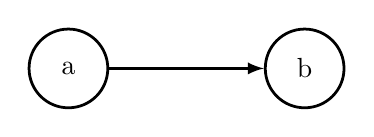
\begin{tikzpicture}
		\node (a) [draw, circle, minimum size=1cm, line width=1pt] {a};
		\node (b) [draw, circle, minimum size=1cm, line width=1pt] at (3,0) {b};
		\draw [-latex, line width=1pt] (a) -- (b);
	\end{tikzpicture}
	\caption{Graphical Model}
	\label{fig:GM}
\end{figure}

\blindtext

\section{Referencing Examples}
\cref{eq:Bayes} shows Bayes' theorem. \cref{fig:GM} depicts a graphical model. The Dirichlet process is discussed in \cite{ferguson1973bayesian}.
	\chapter{Second Chapter}
\blindtext

\section{Bayesian Nonparametrics}
\Blindtext
\Blindtext
\Blindtext
	\bibliography{references.bib}
\end{document}